% Implementation Tables 

\begin{figure*}[h]
    \centering
    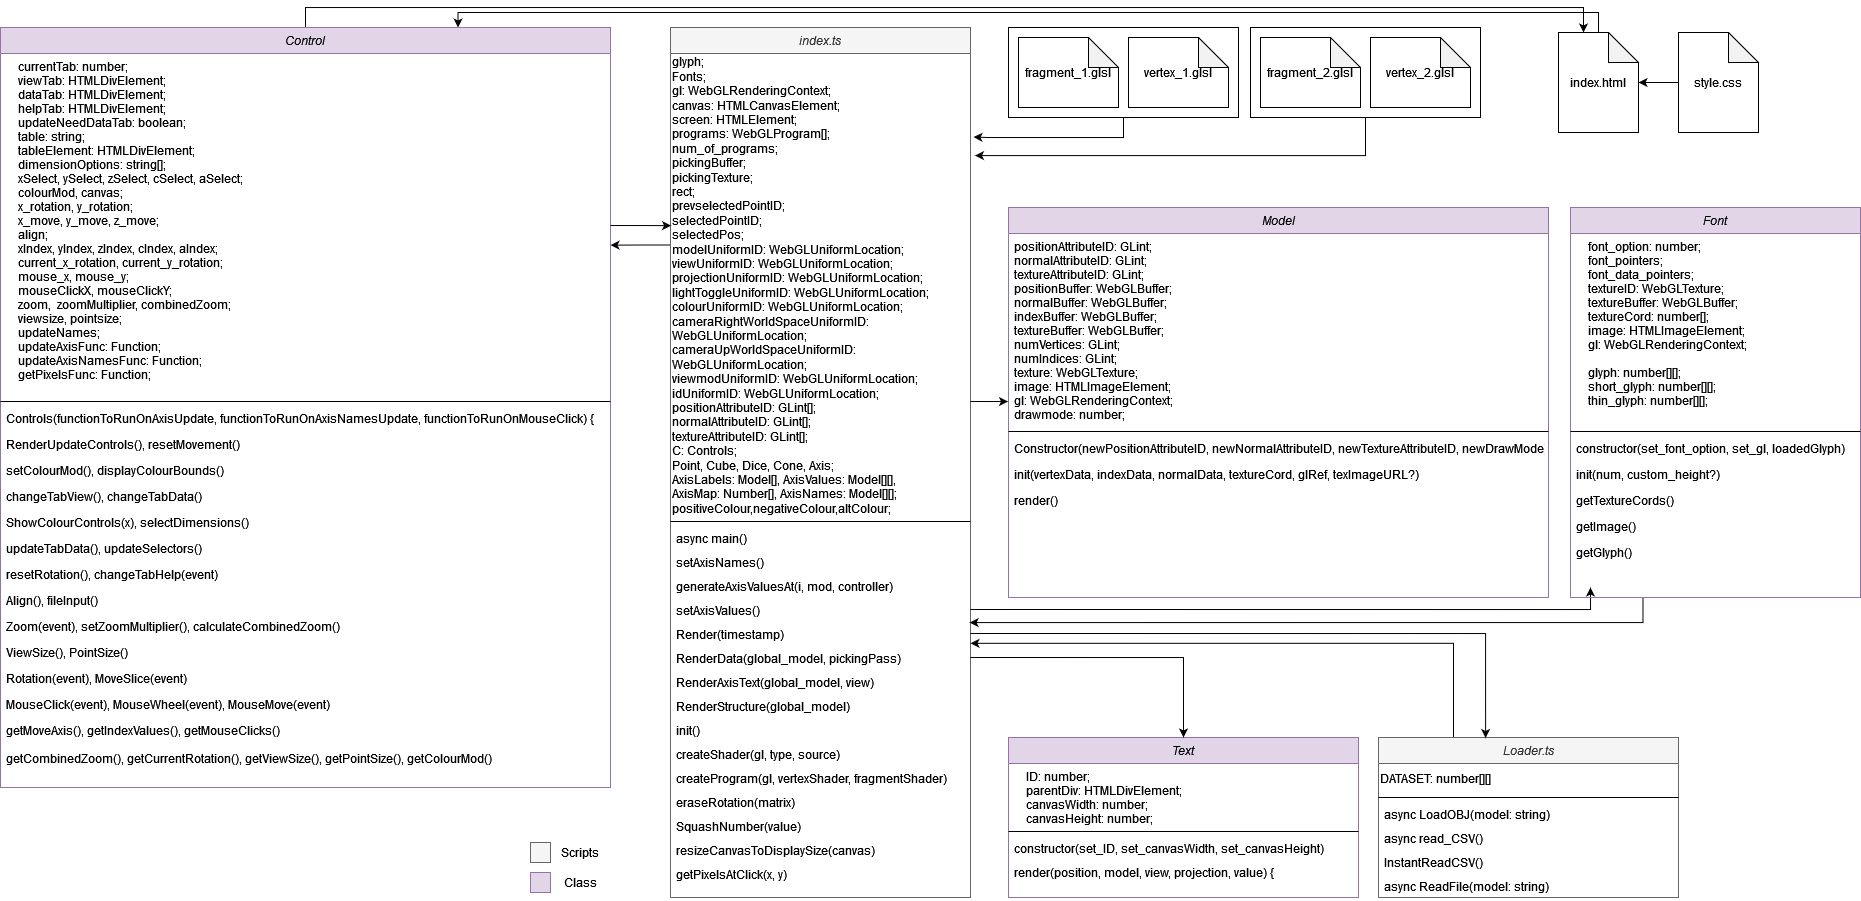
\includegraphics[width=1\textwidth]{author-files/figures/UML_All_fin.drawio.png}
    \caption{UML Diagram - Final App Version}
    \label{fig:graphfin}
\end{figure*}

\begin{table*}[h]
    \begin{tabularx}{\textwidth}{ | X | X | X | }
        \hline
        ID & Title                                                                                               & Estimate (Relative) \\
        \hline
        3  & As a User, I want to be able to view a scatterplot of data set against an axis with accurate scales & 5                   \\
        \hline
        11 & As a User, I want all interactive parts of the Application to be visible at all times               & 1                   \\
        \hline
    \end{tabularx}
    \caption{MVP Feature Set, Sprint 1}
    \label{sprint1}
\end{table*}

\begin{table*}[h]
    \begin{tabularx}{\textwidth}{ | X | X | X | }
        \hline
        ID & Title                                                                                                          & Estimate (Relative) \\
        \hline
        8  & As a User, I want the application to have easy to use on screen controls for interacting with the application  & 3                   \\
        \hline
        1  & As a User, I want to be able to import a dataset into the application to graph it in a 3 dimension scatterplot & 3                   \\
        \hline
        18 & The Axis should scale with the values shown                                                                    & 5                   \\
        \hline
        7  & As a User, I want to be able to rotate the 3D Scatterplot around all 3D axis individually                      & 5                   \\
        \hline
    \end{tabularx}
    \caption{MVP Feature Set, Sprint 2}
    \label{sprint2}
\end{table*}

\begin{table*}[h]
    \begin{tabularx}{\textwidth}{ | X | X | X | }
        \hline
        ID & Title                                                                                                               & Estimate (Relative) \\
        \hline
        2  & As a User, I want to be able to navigate around the generated graph in 3D space while having the axis stay accurate & 6                   \\
        \hline
        5  & As a User, I want to move the 3D view of the scatterplot in 3D using on screen controls                             & 3                   \\
        \hline
        6  & As a User, I want to be able to zoom in and out of the 3D Scatterplot                                               & 10                  \\
        \hline
        9  & As a User, I want to be able to access the application on landscape screens of different sizes                      & 2                   \\
        \hline
        24 & UI doesn't scale very well and not all controls visible                                                             & 3                   \\
        \hline
    \end{tabularx}
    \caption{MVP Feature Set, Sprint 3}
    \label{sprint3}
\end{table*}

\begin{table*}[h]
    \begin{tabularx}{\textwidth}{ | X | X | X | }
        \hline
        ID & Title                                                                                                  & Estimate (Relative) \\
        \hline
        10 & As a User, I want to be able to view instructions within the application on how to use the application & 2                   \\
        \hline
        26 & The User should be able to change the size of the data points                                          & 2                   \\
        \hline
        29 & The User should have the ability to use Mouse Controls for transformation controls                     & 3                   \\
        \hline
        30 & There should be a visible way to identify negative axis values                                         & 3                   \\
        \hline
    \end{tabularx}
    \caption{MVP Feature Set, Sprint 4}
    \label{sprint4}
\end{table*}

\begin{table*}[hbt!]
    \begin{tabularx}{\textwidth}{ | X | X | X | }
        \hline
        ID & Title                                                                               & Estimate (Relative) \\
        \hline
        43 & Refactor Needed (MVC Pattern potential)                                             & 5                   \\
        \hline
        41 & Each Axis should be named / display a name based on the column names in the dataset & 4                   \\
        \hline
    \end{tabularx}
    \caption{Backlog Tasks, Sprint 5}
    \label{sprint5}
\end{table*}

\begin{table*}[hbt!]
    \begin{tabularx}{\textwidth}{ | X | X | X | X | }
        \hline
        ID & Title                                                                                                                                         & Estimate (Relative) & MoSCoW \\
        \hline
        52 & As a Tester, I want data labels to be always visible even when zooming                                                                        & 2                   & Must   \\
        \hline
        54 & Mentioned by Testers, If the slice viewed is not at origin, then using the data zoom should not result in data points moving out of the graph & 5                   & Must   \\
        \hline
        53 & As a Tester, I want to be able to click on a data point and have the value of that point be displayed                                         & 8                   & Must   \\
        \hline
    \end{tabularx}
    \caption{User Testing 1 feature set, Sprint 6}
    \label{sprint6}
\end{table*}

\begin{table*}[hbt!]
    \begin{tabularx}{\textwidth}{ | X | X | X | X | }
        \hline
        ID & Title                                                  & Estimate (Relative) & MoSCoW \\
        \hline
        42 & Create a more robust zoom not limited to only 2 levels & 7                   & Must   \\
        \hline
        70 & Have a Favicon                                         & 1                   & Must   \\
        \hline
    \end{tabularx}
    \caption{Further Improvements feature set, Sprint 6}
    \label{sprint6-2}
\end{table*}

\begin{table*}[hbt!]
    \begin{tabularx}{\textwidth}{ | X | X | X | X | }
        \hline
        ID & Title                                                                                         & Estimate (Relative) & MoSCoW \\
        \hline
        58 & As a Tester, I want to be able to return the graph to it's starting point with a button click & 1                   & Must   \\
        \hline
    \end{tabularx}
    \caption{User Testing 1 feature set, Sprint 7}
    \label{sprint7}
\end{table*}

\begin{table*}[hbt!]
    \begin{tabularx}{\textwidth}{ | X | X | X | X | }
        \hline
        ID & Title                                                                          & Estimate (Relative) & MoSCoW \\
        \hline
        63 & The application should be able to use saturation as an extra dimension         & 6                   & Must   \\
        \hline
        64 & The application should have an option to apply columns to different dimensions & 9                   & Should \\
        \hline
        74 & The application should have a view where the data table can be viewed          & 5                   & Should \\
        \hline
    \end{tabularx}
    \caption{Further Improvements feature set, Sprint 7}
    \label{sprint7-2}
\end{table*}

\begin{table*}[hbt!]
    \begin{tabularx}{\textwidth}{ | X | X | X | X | X | }
        \hline
        ID & Title                                                                                                                    & Estimate (Relative) & MoSCoW & Feature Set    \\
        \hline
        47 & As a Tester, I want to be able to zoom in and out of the graph using the scroll wheel                                    & 1                   & Should & User Testing 1 \\
        \hline
        48 & As a Tester, I want to be able to focus on a single axis through the click of a button- i.e View the graph from one side & 2                   & Should & User Testing 1 \\
        \hline
    \end{tabularx}
    \caption{User Testing 1 feature set, Sprint 8}
    \label{sprint8}
\end{table*}

\begin{table*}[hbt!]
    \begin{tabularx}{\textwidth}{ | X | X | X | X | }
        \hline
        ID & Title                                                                                                          & Estimate (Relative) & MoSCoW \\
        \hline
        50 & As a Tester, I want to be able to view trend lines generated from the data                                     & 10                  & Should \\
        \hline
        51 & As a Tester, I want there to be lines that can help identify the data points location                          & 3                   & Should \\
        \hline
        56 & As a Tester, there should be no performance issues when using Opera                                            & ?                   & Should \\
        \hline
        57 & As a Tester, Graph fully doesn't render in rare cases                                                          & ?                   & Must   \\
        \hline
        60 & As a Tester, I want to be able to highlight multiple data points to more easily track patterns                 & 4                   & Could  \\
        \hline
        55 & As a Tester, Nodes should not overlap                                                                          & ?                   & Could  \\
        \hline
        49 & As a Tester, I want to be able to search for a specific point- such as "Find a point above x = 5 if it exists" & 10                  & Could  \\
        \hline
    \end{tabularx}
    \caption{User Testing 1 feature set, Stories not implemented}
    \label{UT1}
\end{table*}

\begin{table*}[hbt!]
    \begin{tabularx}{\textwidth}{ | X | X | X | X | }
        \hline
        ID & Title                                                                                                               & Estimate (Relative) & MoSCoW \\
        \hline
        81 & As a Tester, The mouse zoom should be flipped to scroll up to zoom in and scroll down to zoom out                   & 1                   & Must   \\
        \hline
        82 & There is a chance that axis titles get stuck and don't update when another file is input                            & 3                   & Must   \\
        \hline
        83 & As a Tester, I would like better performance with large datasets to better concentrate                              & 10                  & Should \\
        \hline
        84 & As a Tester, I would like data points with saturation to be outlined to be easier to see                            & 4                   & Should \\
        \hline
        85 & Fix bugs with picking, not accurate and jumps back to a point when nothing is selected                              & 2                   & Must   \\
        \hline
        86 & Files are still uploaded if they are not CSV, have it so name of failed to upload file is not shown                 & 1                   & Must   \\
        \hline
        87 & Labels Flicker bug                                                                                                  & 8                   & Must   \\
        \hline
        88 & Labels are not clipped correctly, remaining dots                                                                    & 5                   & Must   \\
        \hline
        89 & Headers in Data Management do not match with table                                                                  & 2                   & Must   \\
        \hline
        90 & As a Tester, I would like to use full Colour as a dimension                                                         & 5                   & Should \\
        \hline
        91 & As a Tester, I would like scroll bars to rotate the camera                                                          & 2                   & Could  \\
        \hline
        93 & As a tester, I would like a "Feature Finder" that zooms into where data is if it's beyond the current view position & 7                   & Should \\
        \hline
    \end{tabularx}
    \caption{User Testing 2 feature set, Stories not implemented}
    \label{UT2}
\end{table*}

\begin{table*}[hbt!]
    \begin{tabularx}{\textwidth}{ | X | X | X | X | }
        \hline
        ID  & Title                                                                                               & Estimate (Relative) & MoSCoW \\
        \hline
        94  & Research and integrate a Modern UI framework or library to handle state and UI component management & 10                  & Must   \\
        \hline
        95  & Optimize Model Class for higher performance                                                         & 5                   & Must   \\
        \hline
        96  & Identify and fix any bugs causing inaccuracy in what point is selected                              & 6                   & Must   \\
        \hline
        97  & Fix Fragment shader bugs causing unclear text                                                       & 4                   & Must   \\
        \hline
        98  & Research SDF font's for clearer text                                                                & 5                   & Could  \\
        \hline
        99  & Create Clearer Instructions for the 4th dimension controls                                          & 3                   & Must   \\
        \hline
        100 & Look into opportunities to rework how the 4th dimension controls work                               & 5                   & Should \\
        \hline
    \end{tabularx}
    \caption{Further Improvements feature set, Stories not implemented}
    \label{FI2}
\end{table*}
